\FloatBarrier

\begin{figure}[h!]
	\centering
	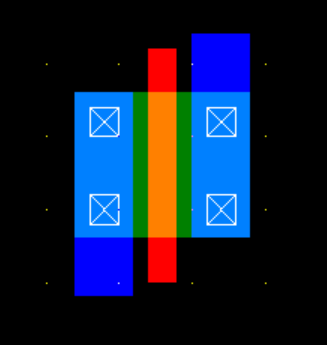
\includegraphics[scale=0.75]{../images/nmos.PNG}
	\caption{NMOS Layout}
	\label{fig:nmos}
\end{figure}

\FloatBarrier

Figure (\ref{fig:nmos}) shows an NMOS transistor's layout. Figure (\ref{fig:l1_mos}) depicts the $I_{DS}$ versus $V_{DS}$ curve of the level 1 NMOS model.

\FloatBarrier

\begin{figure}[h!]
	\centering
	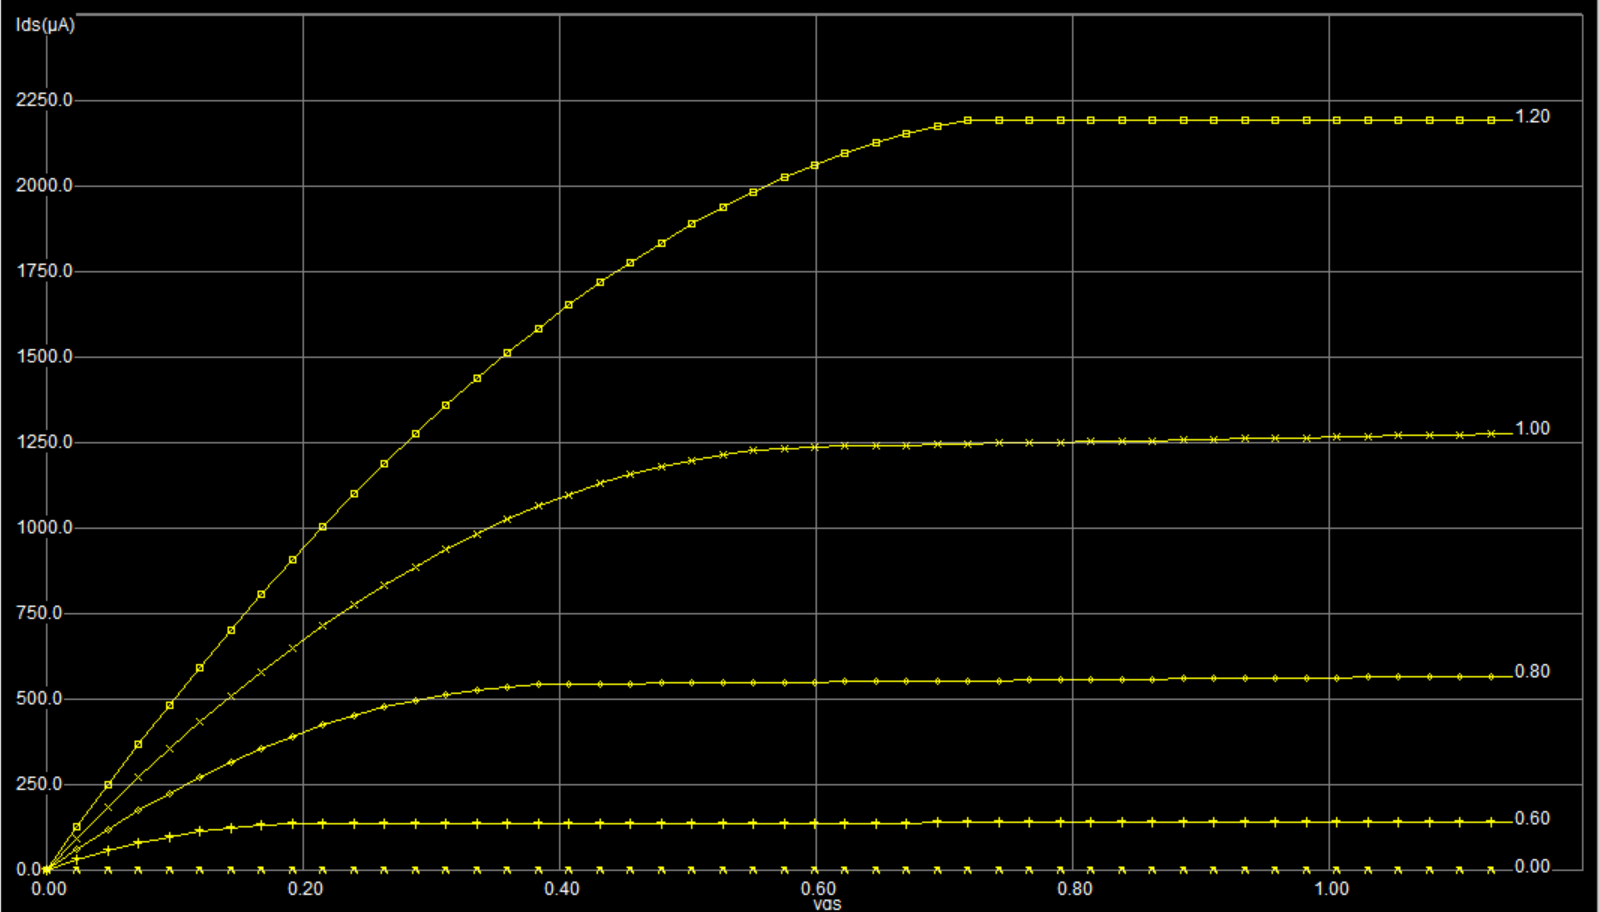
\includegraphics[scale=0.75]{../images/l1_mos.PNG}
	\caption{Level 1 NMOS Model}
	\label{fig:l1_mos}
\end{figure}

\FloatBarrier

The L1 NMOS model is a standard transistor model that neglects channel length modulation.
When $V_{DS} = V_{GS} - V_{T}$, the current tapers off, and the MOSFET enters the saturation region.

\FloatBarrier

\begin{figure}[h!]
	\centering
	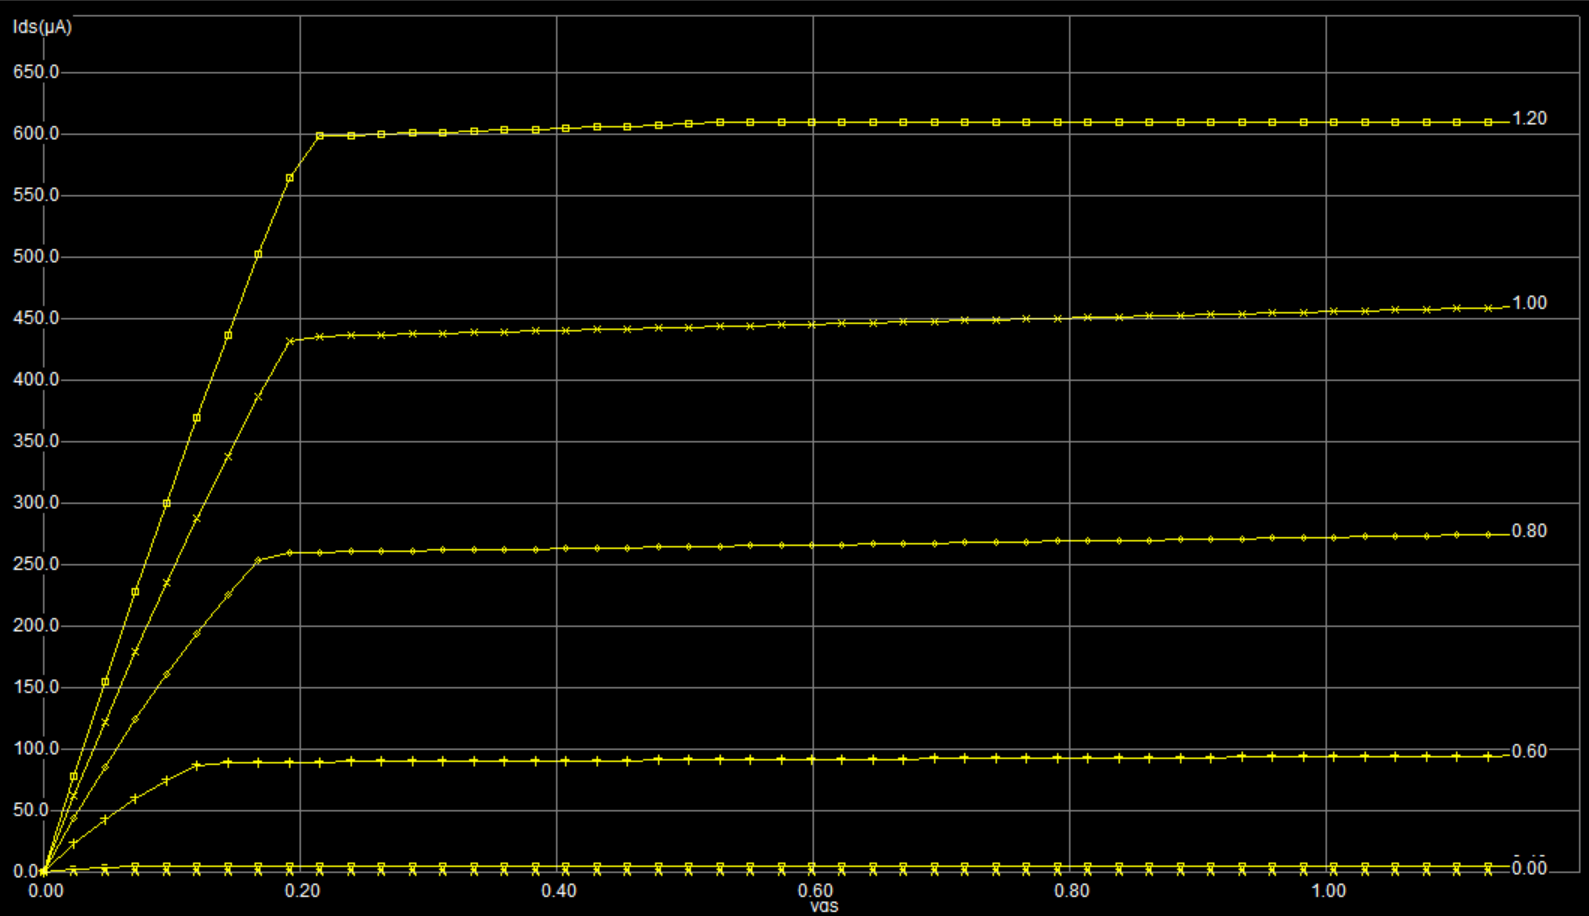
\includegraphics[scale=0.75]{../images/l3_mos.PNG}
	\caption{Level 3 NMOS Model}
	\label{fig:l3_mos}
\end{figure}

\FloatBarrier

L3 is an improvement that accounts for effects that cause the transistor to enter saturation at lower voltages.
This may be a short-channel effect in integrated circuits.
If the channel is sufficiently short, the depletion regions at the source and drains can extend into the channel.
As a result, the transistor may enter saturation at lower voltages since the depletion regions extend into the channel at higher drain voltages in saturation.
This is the cause of channel length modulation, though the level 3 model does not account for that effect specifically.

\FloatBarrier

\begin{figure}[h!]
	\centering
	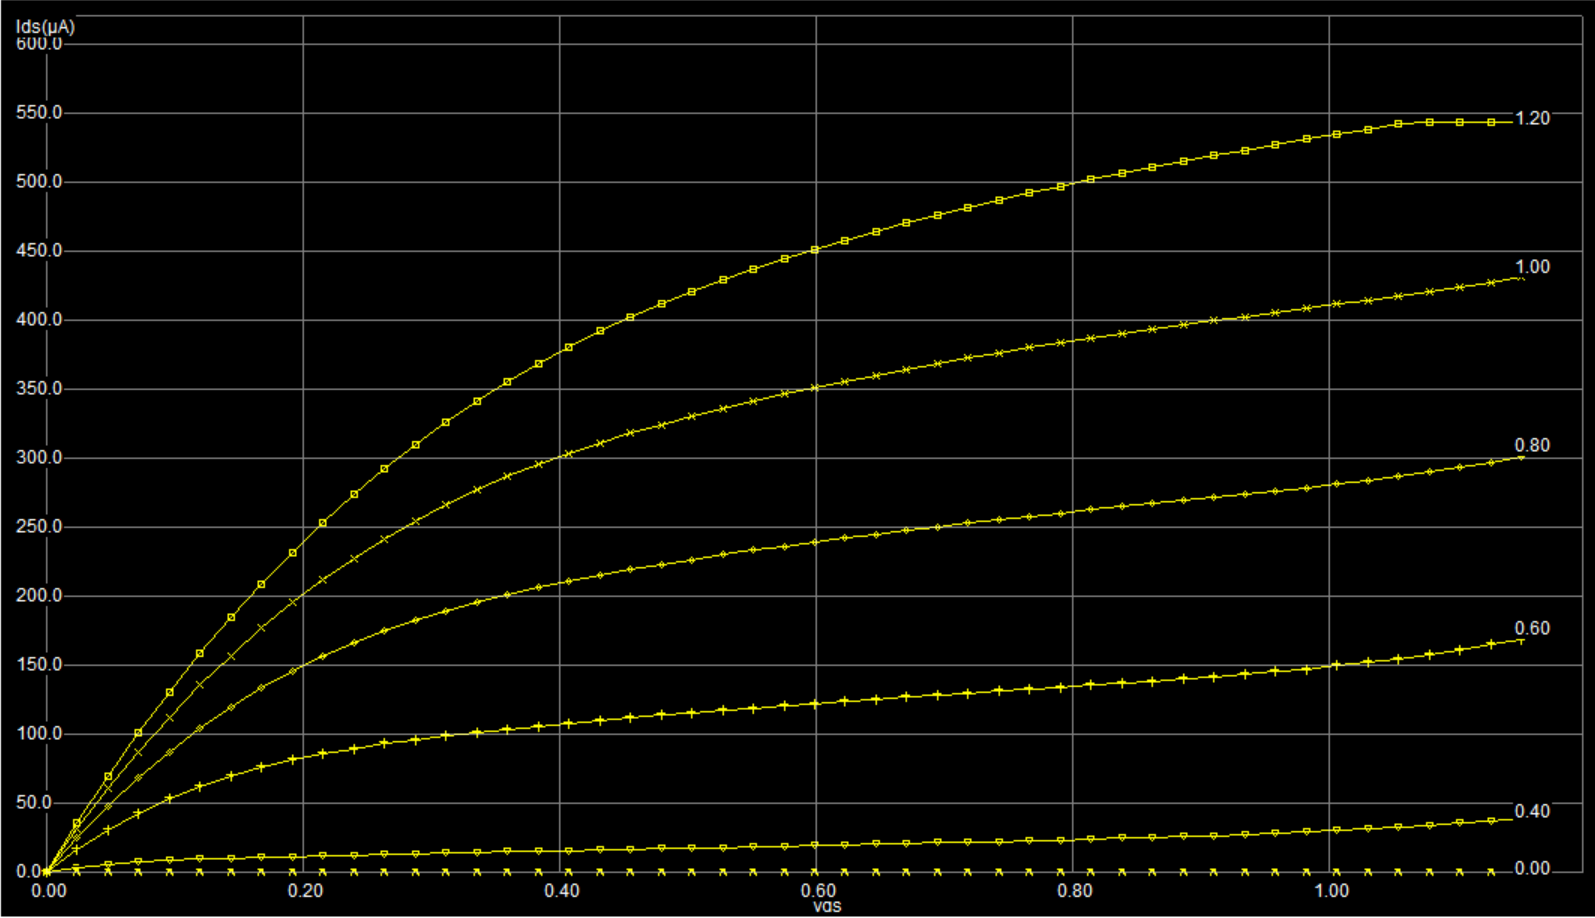
\includegraphics[scale=0.75]{../images/bsim4_mos.PNG}
	\caption{BSIM4 NMOS Model}
	\label{fig:bsim4_mos}
\end{figure}

\FloatBarrier

The BSIM4 model accounts for channel length modulation, which explains why the current increases linearly with $V_{DS}$ in saturation.
The SPICE model typically used in prior simulations accounts for channel length modulation, like in the BSIM4 model.
It also contains information on junction capacitances and other parasitics, like gate-drain overlap.
Therefore, the SPICE model currently used in labs is probably closer to the level of accuracy of the BSIM4 model, meaning that the SPICE model used hitherto is quite accurate.
It could potentially be used to model some sub-micrometer scale integrated circuit transistors, though may not be adequate for deep submicron processes, like a modern FinFET process. \\

The body effect in a MOSFET occurs when the body is not grounded.
Typically, the body is set to the lowest voltage in the circuit.
However, if the body's voltage is increased, the MOS capacitor must now have its gate set to a higher voltage to ensure that the channel is properly formed.
Therefore, the threshold voltage increases as the body voltage is increased.
This is evident from the transistor models.

\FloatBarrier

\begin{figure}[h!]
	\centering
	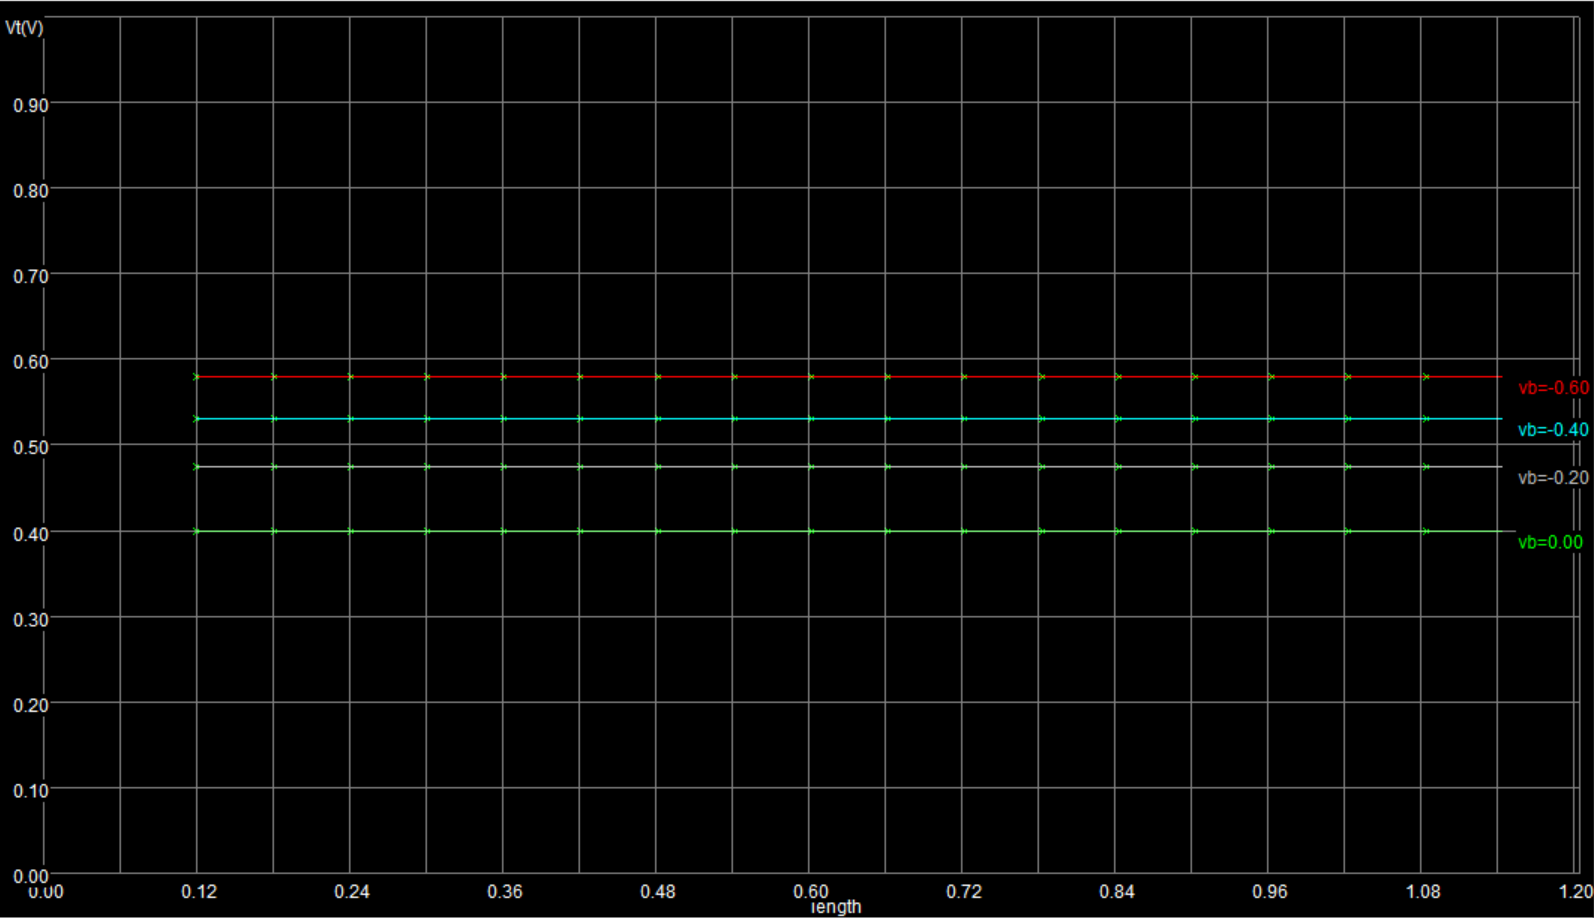
\includegraphics[scale=0.75]{../images/l1_bodyeffect.PNG}
	\caption{L1 NMOS Body Effect}
	\label{fig:l1_bodyeffect}
\end{figure}

\FloatBarrier

\FloatBarrier

\begin{figure}[h!]
	\centering
	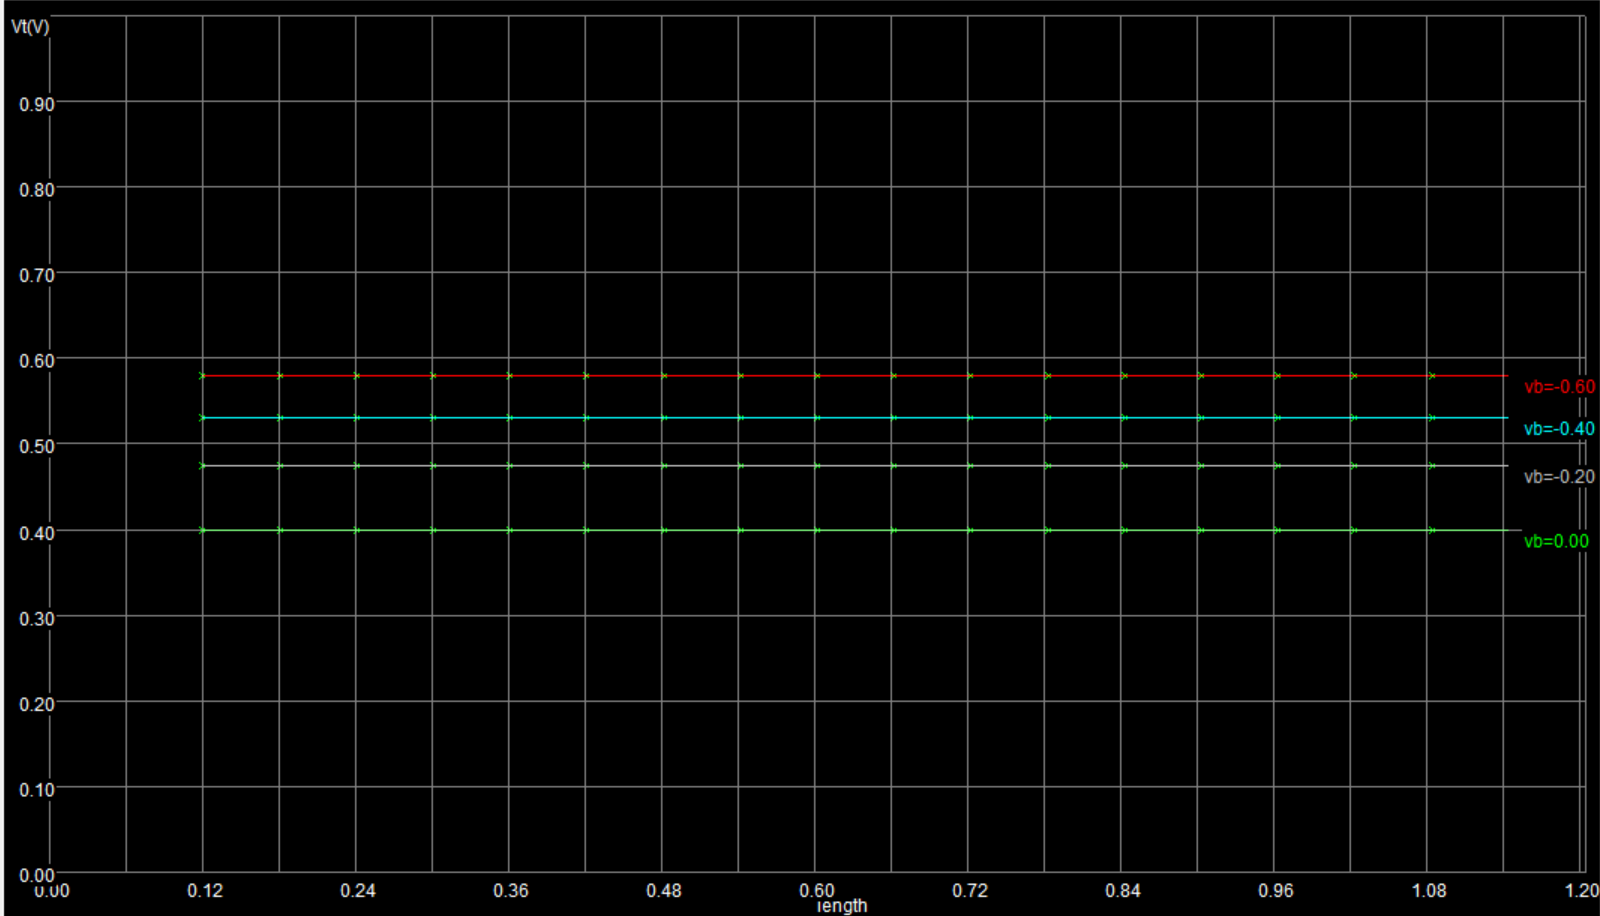
\includegraphics[scale=0.75]{../images/l3_bodyeffect.PNG}
	\caption{L3 NMOS Body Effect}
	\label{fig:l3_bodyeffect}
\end{figure}

\FloatBarrier

The body effect observed in figures (\ref{fig:l1_bodyeffect}) and (\ref{fig:l3_bodyeffect}) is essentially the same.
Increasing the body voltage increases the threshold voltage.
In neither of these models does the body effect depend on the channel length.

\FloatBarrier

\begin{figure}[h!]
	\centering
	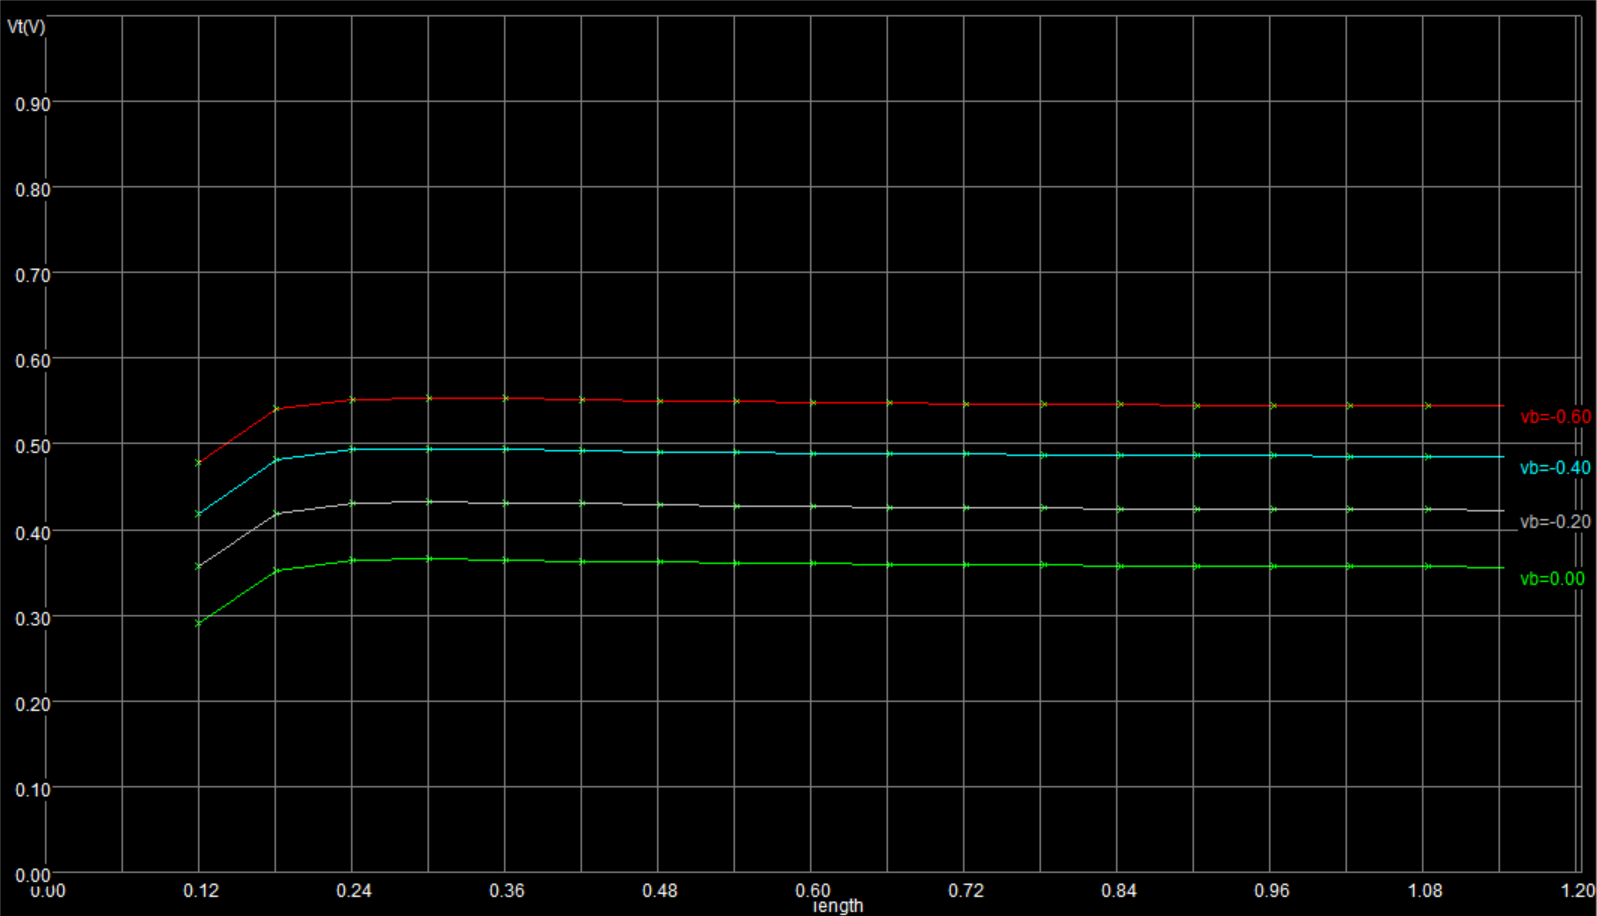
\includegraphics[scale=0.75]{../images/bsim4_bodyeffect.PNG}
	\caption{BSIM4 NMOS Body Effect}
	\label{fig:bsim4_bodyeffect}
\end{figure}

\FloatBarrier

The BSIM4 model accounts for effects that occur in submicron processes when the channel length becomes very short.
The threshold voltage drops when the channel length is very short.
This might be because the depletion layers from the source and the drain help facilitate the motion of charges in the channel, meaning fewer charges are required to sustain an adequate current.
The SPICE model does not seem to contain information on such short-channel effects, but does contain information about junction capacitances with the body, meaning that it probably accounts for some body effects. \\

If the oxide layer thickness is increased, the MOS capacitor's capacitance is decreased.
Thus, for the same applied gate voltage, less charge accumulates in the channel.
Therefore, ceteris paribus, the current should decrease if the oxide layer thickness is increased. \\

\FloatBarrier

\begin{figure}[h!]
	\centering
	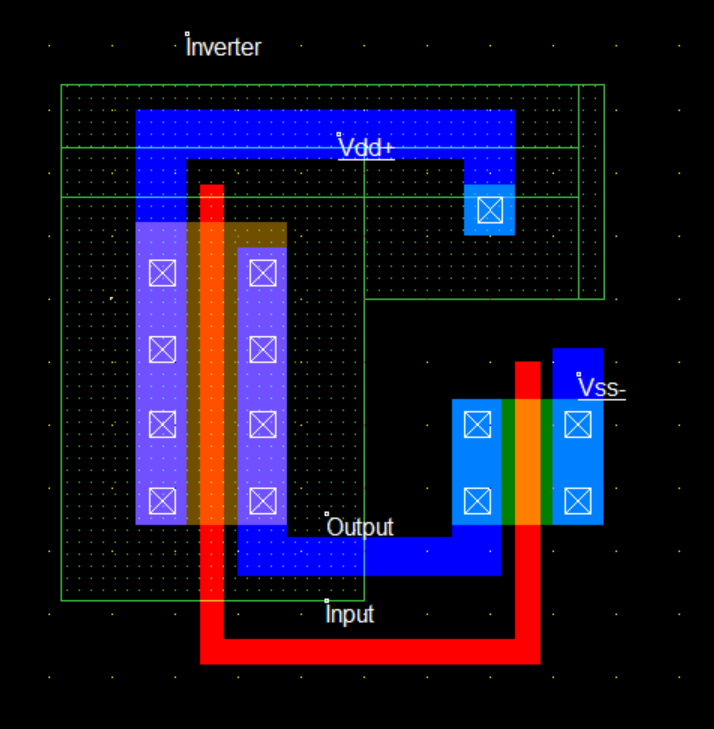
\includegraphics[scale=0.75]{../images/inverter_layout.PNG}
	\caption{Layout of CMOS Inverter}
	\label{fig:inverter_layout}
\end{figure}

\FloatBarrier

The CMOS inverter can be implemented in a true integrated circuit process, depicted in figure (\ref{fig:inverter_layout}).
The design depicted passes the design rule check.

\FloatBarrier

\begin{figure}[h!]
	\centering
	\includegraphics[scale=0.75]{../images/cmos_layout_transient.PNG}
	\caption{CMOS Inverter Layout Transient Response}
	\label{fig:cmos_layout_transient}
\end{figure}

\FloatBarrier

\FloatBarrier

\begin{figure}[h!]
	\centering
	\includegraphics[scale=0.75]{../images/cmos_layout_vtc.PNG}
	\caption{CMOS Inverter Layout Voltage Transfer Characteristic (VTC)}
	\label{fig:cmos_layout_vtc}
\end{figure}

\FloatBarrier

Figure (\ref{fig:cmos_layout_transient}) presents the transient response of the inverter.
Figure (\ref{fig:cmos_layout_vtc}) depicts the voltage transfer characteristic.
The nature of the results is similar to those presented in SPICE simulations earlier.

